\documentclass[a4paper,12pt]{article}

% Paquetes básicos
\usepackage[utf8]{inputenc}
\usepackage[T1]{fontenc}
\usepackage[spanish]{babel}
\usepackage{graphicx}
\usepackage{xcolor}
\usepackage{lipsum}
\usepackage{geometry}
\geometry{top=3cm, bottom=3cm, left=2.5cm, right=2.5cm}

% Paquetes para diseño
\usepackage{titlesec}
\usepackage{fancyhdr}
\usepackage{amsmath}
\usepackage{amssymb}
\usepackage{hyperref}

% Paquetes para el entorno lstlisting
\usepackage{listings}
\usepackage{inconsolata}

\usepackage{float}

%encabezado y pie de página nivel profesional
\usepackage{fancyhdr}
\pagestyle{fancy}
\fancyhf{}
\fancyhead[L]{\leftmark}
\fancyhead[R]{\rightmark}
\fancyfoot[C]{\thepage}
\fancyfoot[R]{\textbf{(UGR)} \today}
\renewcommand{\headrulewidth}{0.4pt}
\renewcommand{\footrulewidth}{0.4pt}
\setlength{\headheight}{15pt}
\setlength{\headsep}{10pt}
\setlength{\footskip}{20pt}
\usepackage{truncate}
\fancyhead[L]{\truncate{0.5\headwidth}{\leftmark}}
\fancyhead[R]{\truncate{0.5\headwidth}{\rightmark}}
\usepackage{mathpazo}

% Paquete para fondo
\usepackage{background}

% Configuración de lstlisting
\lstset{
    inputencoding=utf8,          % Permite UTF-8
    extendedchars=true,          % Reconoce caracteres extendidos
    literate=                    % Configuración manual para tildes y símbolos
        {á}{{\'a}}1
        {é}{{\'e}}1
        {í}{{\'i}}1
        {ó}{{\'o}}1
        {ú}{{\'u}}1
        {ñ}{{\~n}}1
        {Á}{{\'A}}1
        {É}{{\'E}}1
        {Í}{{\'I}}1
        {Ó}{{\'O}}1
        {Ú}{{\'U}}1
        {Ñ}{{\~N}}1
        {¿}{{\textquestiondown}}1
        {¡}{{\textexclamdown}}1,
    basicstyle=\ttfamily,        % Fuente monoespaciada
    breaklines=true,             % Habilita salto de línea automático
    frame=single,                % Marco alrededor del código
    backgroundcolor=\color{gray!10}, % Fondo gris claro
    keywordstyle=\color{blue},   % Color para palabras clave
    commentstyle=\color{green},  % Color para comentarios
    stringstyle=\color{red}      % Color para strings
}
\lstdefinestyle{customcpp}{
    language=C++,                % Lenguaje de programación
    showspaces=false,            % No mostrar espacios
    showtabs=false,              % No mostrar tabulaciones
    tabsize=4,                   % Tamaño de tabulación
    showstringspaces=false,      % No mostrar espacios en strings
    numbers=left,                % Números de línea a la izquierda
    numberstyle=\tiny\color{gray}, % Estilo de los números de línea
    numbersep=5pt,               % Separación de los números de línea
    stepnumber=1,                % Mostrar número en cada línea
    basicstyle=\ttfamily\footnotesize, % Estilo básico del código
    keywordstyle=\bfseries\color{blue}, % Estilo de las palabras clave
    commentstyle=\itshape\color{green!50!black}, % Estilo de los comentarios
    stringstyle=\color{red},     % Estilo de los strings
    identifierstyle=\color{black}, % Estilo de los identificadores
    % procnamekeys={def,class},    % Palabras clave para nombres de funciones
    morekeywords={constexpr,nullptr,size_t}, % Más palabras clave
    emph={int,char,double,float,unsigned}, % Palabras a enfatizar
    emphstyle=\color{magenta},   % Estilo de las palabras enfatizadas
    backgroundcolor=\color{gray!10}, % Color de fondo
    frame=shadowbox,             % Marco con sombra
    rulesepcolor=\color{gray},   % Color de la línea de separación
    breakatwhitespace=false,     % No cortar en espacios en blanco
    breaklines=true,             % Cortar líneas largas
    captionpos=b,                % Posición del título (abajo)
    escapeinside={(*@}{@*)},     % Delimitadores para escapar a LaTeX
    morecomment=[l][\color{magenta}]{\#}, % Comentarios de una línea
    morecomment=[s][\color{orange}]{/*}{*/}, % Comentarios multilínea
    morestring=[b]",             % Strings entre comillas dobles
    morestring=[b]'              % Strings entre comillas simples
}

% Configuración de título
\titleformat{\section}{\normalfont\Large\bfseries}{\thesection}{1em}{}

% Información del documento
\title{
    \vspace{-2cm}
    
\includegraphics[width=0.3\textwidth]{images/etsiit.png} \\ % Cambia el logo si es necesario
    \LARGE Ingeniería Informática + ADE\\
    \large Universidad de Granada (UGR)\\[1cm]
}
\author{\textbf{Autor:} Ismael Sallami Moreno}
\date{\textbf{Asignatura:} Apuntes Sistemas Concurrentes y Distribuidos (SCD)\\[1cm]}

% Configuración del fondo
\backgroundsetup{
    scale=1,
    color=black,
    opacity=0.2,
    angle=0,
    position=current page.south,
    vshift=0pt,
    hshift=0pt,
    contents={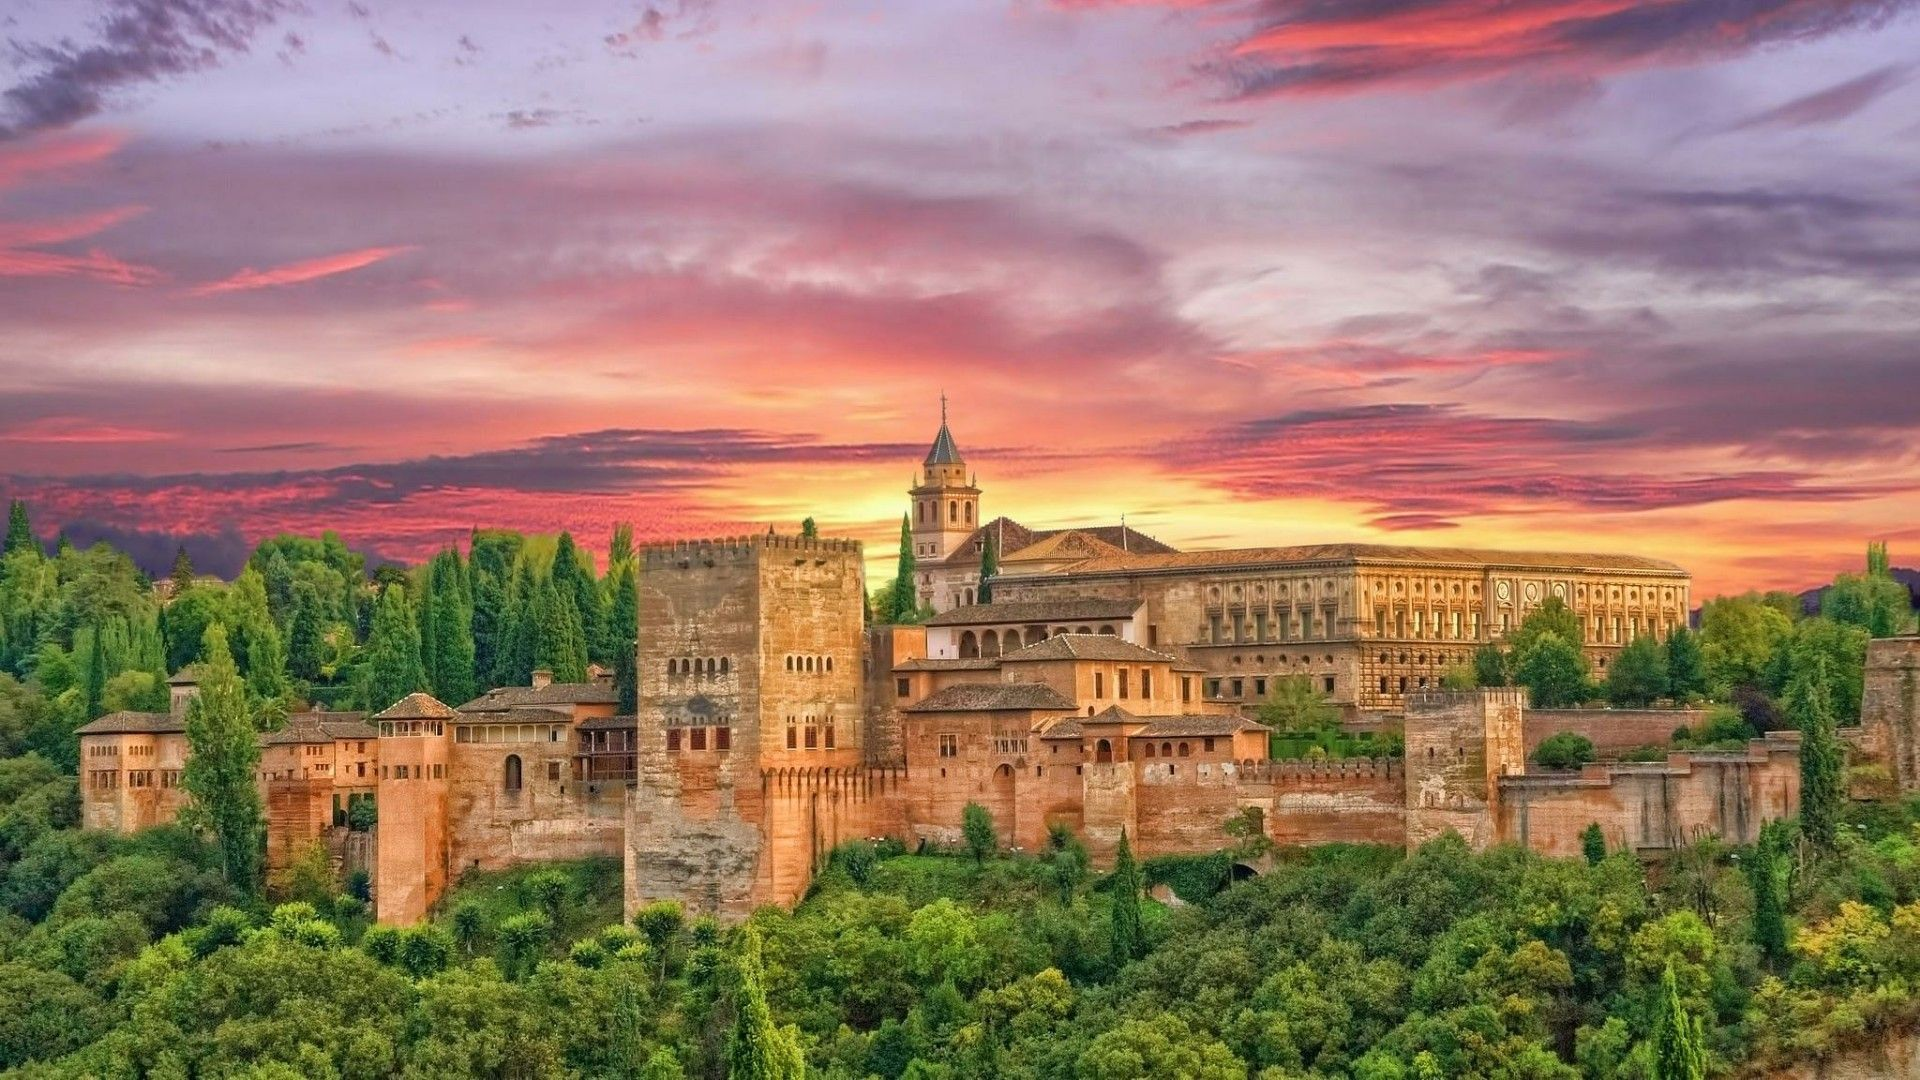
\includegraphics[width=\paperwidth,height=\paperheight,keepaspectratio]{images/granada.jpg}}
}

% Inicio del documento
\begin{document}

% Portada
\maketitle
\thispagestyle{empty}

\begin{center}
    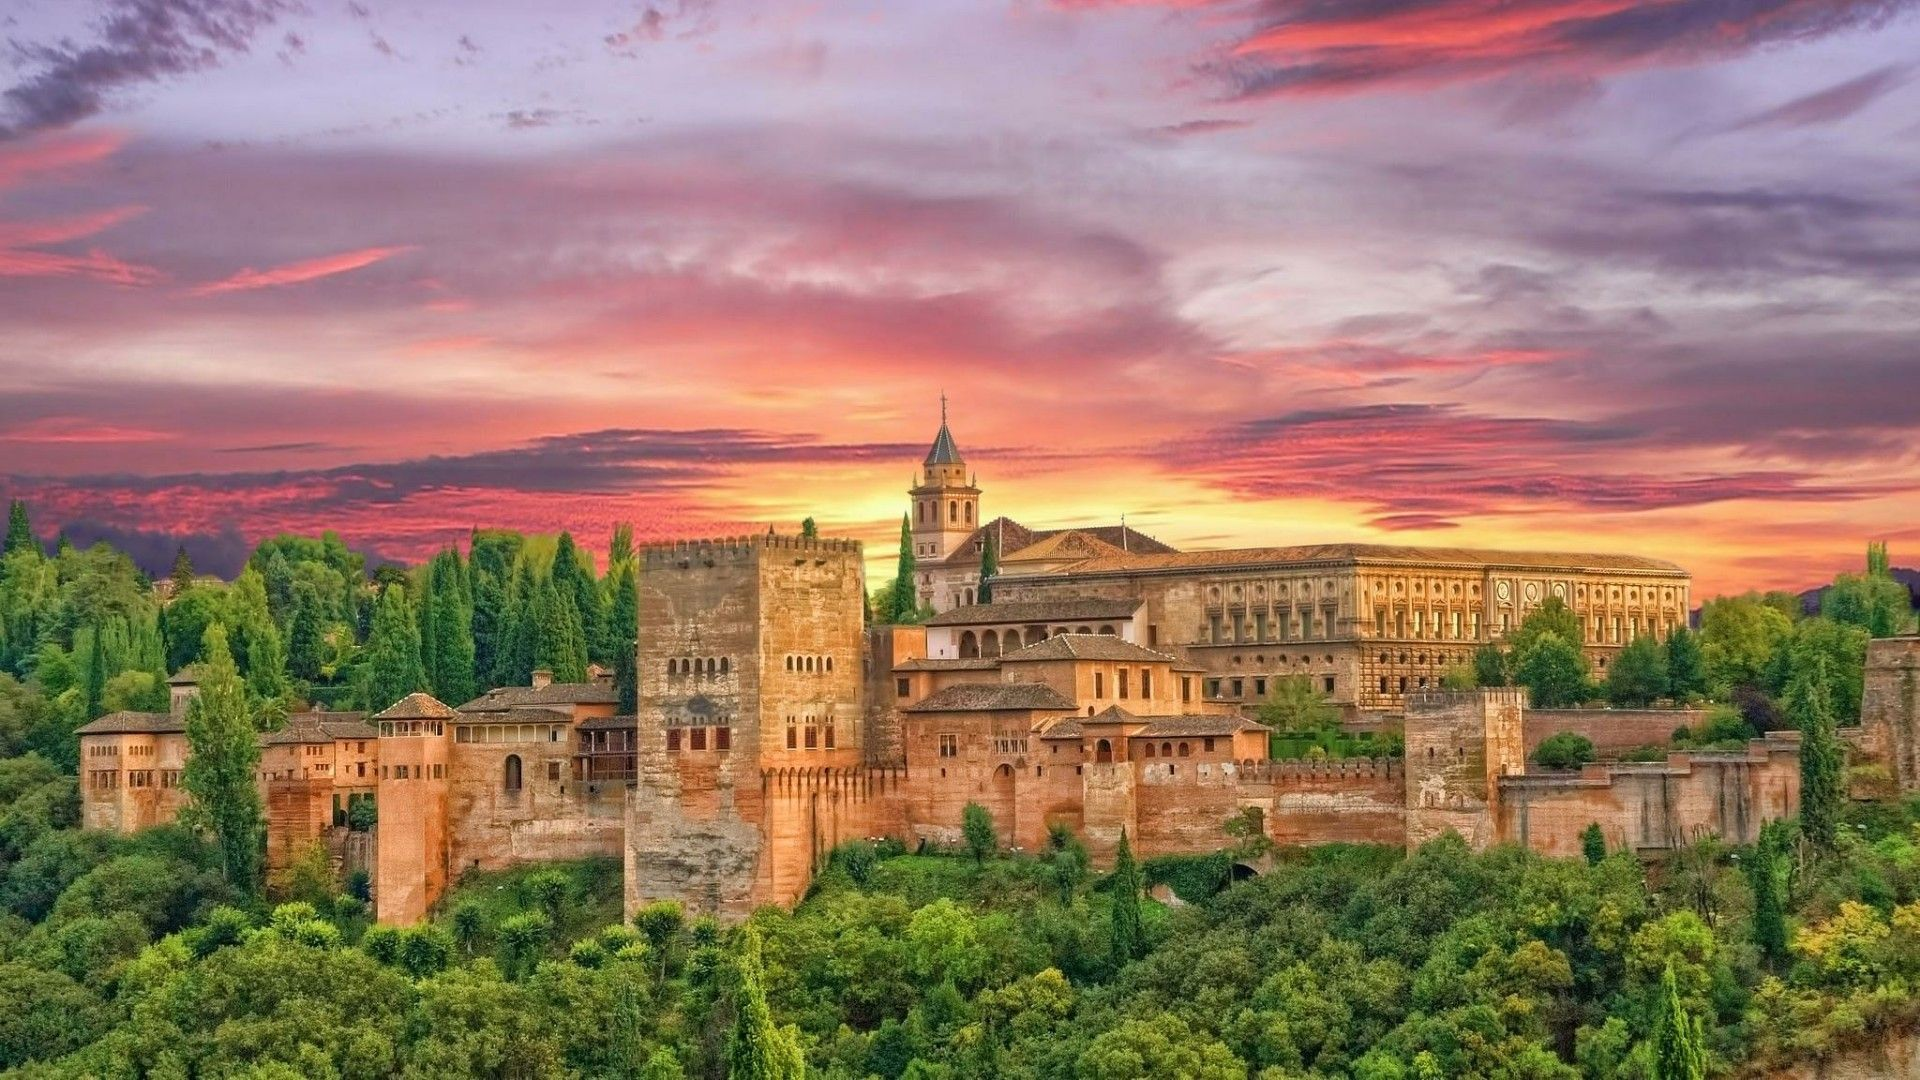
\includegraphics[width=\textwidth,height=0.4\textheight,keepaspectratio]{images/granada.jpg} \\ % Añade tu imagen de fondo
    \vfill
\end{center}

\newpage

% Índice (opcional)
\tableofcontents
\newpage

\section{Tema 3: Sistemas basados en el paso de mensajes}

\subsection{El cuello de botella de Von Neumann}

El \textbf{cuello de botella de Von Neumann} se refiere a una limitación inherente en las arquitecturas de computación clásicas basadas en el modelo de programa único almacenado. Este problema surge debido a la dependencia de un único bus para transferir datos e instrucciones entre la memoria y la unidad de procesamiento central (CPU). A continuación, se presentan sus principales características y consecuencias:

\begin{itemize}
    \item \textbf{Limitación de velocidad del bus:} La transferencia de datos entre la memoria y la CPU está restringida por la velocidad máxima del bus, lo que afecta el rendimiento general del sistema.
    \item \textbf{Cuello de botella:} Dado que no es posible realizar simultáneamente una operación de búsqueda de instrucciones y una operación de datos, se genera un retraso en el flujo de ejecución de las instrucciones.
    \item \textbf{Impacto en el rendimiento:} Esta arquitectura requiere más tiempo de ejecución para los programas, lo que reduce la eficiencia del sistema computacional.
\end{itemize}

El cuello de botella de Von Neumann es una de las razones principales por las cuales las arquitecturas modernas buscan soluciones más eficientes, como los sistemas multiprocesadores o arquitecturas paralelas.

\subsection{Clasificación de Flynn}

La \textbf{clasificación de Flynn} es un esquema que categoriza las arquitecturas de sistemas computacionales en función de cómo manejan las instrucciones y los datos durante la ejecución. Esta clasificación es fundamental para entender los diferentes modelos de procesamiento y se divide en cuatro categorías principales:

\begin{itemize}
    \item \textbf{SISD (Single Instruction, Single Data):} 
    \begin{itemize}
        \item Una sola unidad de control ejecuta una única secuencia de instrucciones.
        \item Procesa un único flujo de datos.
        \item Ejemplo: computadores monoprocesador tradicionales.
    \end{itemize}

    \item \textbf{SIMD (Single Instruction, Multiple Data):}
    \begin{itemize}
        \item Una única instrucción se aplica simultáneamente a múltiples flujos de datos.
        \item Común en aplicaciones con operaciones repetitivas sobre grandes conjuntos de datos, como gráficos y procesamiento de señales.
        \item Ejemplo: procesadores vectoriales y GPU.
    \end{itemize}

    \item \textbf{MISD (Multiple Instruction, Single Data):}
    \begin{itemize}
        \item Múltiples unidades de control ejecutan distintas instrucciones sobre un único flujo de datos.
        \item Es menos común en sistemas reales debido a limitaciones prácticas.
    \end{itemize}

    \item \textbf{MIMD (Multiple Instruction, Multiple Data):}
    \begin{itemize}
        \item Múltiples unidades de control ejecutan distintas secuencias de instrucciones sobre múltiples flujos de datos.
        \item Flexible y utilizado en sistemas paralelos modernos.
        \item Ejemplo: arquitecturas multicore y clusters de computadoras.
    \end{itemize}
\end{itemize}

Esta clasificación permite identificar las capacidades y limitaciones de las diferentes arquitecturas, sirviendo como guía para diseñar y optimizar sistemas computacionales.

%https://chatgpt.com/c/676941fc-2ae8-8012-afcb-4f356a5273ee

\subsection{Diferencias entre Multiprocesador SMP y AMP}

\begin{table}[H]
\centering
\begin{tabular}{|p{4cm}|p{6cm}|p{5cm}|}
\hline
\textbf{Características}        & \textbf{SMP (Multiprocesamiento Simétrico)}  & \textbf{AMP (Multiprocesamiento Asimétrico)}  \\ \hline
\textbf{Arquitectura}           & Todos los procesadores son iguales y comparten el acceso a la memoria & Un procesador principal controla el sistema y los otros son secundarios  \\ \hline
\textbf{Acceso a memoria}       & Todos los procesadores tienen acceso compartido a la memoria central  & Solo el procesador principal tiene acceso a la memoria central  \\ \hline
\textbf{Control de procesos}    & Los procesadores pueden trabajar independientemente & El procesador principal gestiona los procesos y asigna tareas a los secundarios \\ \hline
\textbf{Escalabilidad}          & Alta escalabilidad; se pueden agregar más procesadores sin mucha complicación  & Baja escalabilidad; añadir más procesadores no mejora el rendimiento de forma eficiente \\ \hline
\textbf{Costo}                  & Más costoso debido a la necesidad de múltiples procesadores iguales y una memoria compartida  & Menos costoso, ya que solo se necesita un procesador principal y algunos secundarios \\ \hline
\textbf{Rendimiento}            & Mejor rendimiento en tareas paralelas y de procesamiento intensivo  & Menor rendimiento en tareas paralelas, debido a la dependencia del procesador principal \\ \hline
\textbf{Sistemas típicos}       & Servidores, estaciones de trabajo y sistemas de alta gama  & Sistemas embebidos, estaciones de trabajo de menor escala y dispositivos con recursos limitados \\ \hline
\end{tabular}
\caption{Diferencias entre Multiprocesador SMP y AMP}
\end{table}


\subsection{Mecanismo de citas}

Se trata de una operación de comunicación NO bloqueante y sin búfer. La cita tiene lugar antes de que comience la transmisión de datos.

\subsection{Paso de mensajes bloqueante con búfer}

El proceso emisor vuelve inmediatamente al ejecutar la operación de envío, \textit{salvo que el proceso buffer esté lleno}. En este caso, el proceso emisor se bloquea hasta que haya espacio en el buffer. La operación \textit{receive} no vuelve hasta que se han recibido los datos.

\subsection{Paso de mensajes no bloqueante con búfer}

En este caso se reduce el tiempo de espera debido a que la operación \textit{receive} provoca la transferencia inmediata de datos del búfer a la memoria del proceso receptor.

\subsection{MPI}
\subsubsection{Comunicación bloqueante}
\subsubsection*{Campos de operación MPI de envío con buffer}
\begin{lstlisting}[language=c++]
int MPI_Send(void *buf, int count, MPI_Datatype datatype, int dest, int tag, MPI_Comm comm);
\end{lstlisting}
\subsubsection*{Campos de operación MPI de recepción con buffer}
\begin{lstlisting}[language=c++]
int MPI_Recv(void *buf, int count, MPI_Datatype datatype, int source, int tag, MPI_Comm comm, MPI_Status *status);
\end{lstlisting}

\begin{itemize}
    \item El \textit{origen, tag, comunicador} deben de coincidir en el mensaje enviado y recibido.
    \item \textit{MPI\_Send, MPI\_Recv, MPI\_Ssend} no vuelven hasta que se completan.
\end{itemize}

\subsubsection{Comunicación No bloqueante}
\begin{itemize}
    \item \textit{MPI\_Isend, MPI\_Irecv, MPI\_Iprobe, MPI\_Test} son operaciones no bloqueantes.
\begin{itemize}
    \item \textit{MPI\_Isend:} Inicia una operación de envío no bloqueante. Permite que el programa continúe ejecutándose mientras se realiza la operación de envío en segundo plano.
    \item \textit{MPI\_Irecv:} Inicia una operación de recepción no bloqueante. Permite que el programa continúe ejecutándose mientras se realiza la operación de recepción en segundo plano.
    \item \textit{MPI\_Iprobe:} Permite comprobar de manera no bloqueante si hay un mensaje disponible para ser recibido. Esto es útil para evitar que el programa se bloquee esperando un mensaje.
    \item \textit{MPI\_Test:} Verifica si una operación no bloqueante ha completado. Esto permite al programa comprobar el estado de las operaciones no bloqueantes y actuar en consecuencia.
\end{itemize}
\end{itemize}

\subsubsection{Sondeo de Mensajes}
\begin{itemize}
    \item \textit{MPI\_Iprobe} y \textit{MPI\_Probe} son operaciones de sondeo de mensajes que permiten a un proceso verificar si hay mensajes disponibles para ser recibidos.
    \begin{itemize}
        \item \textit{MPI\_Iprobe:} Permite sondear de manera no bloqueante si hay mensajes disponibles para ser recibidos. Devuelve un valor verdadero si hay mensajes pendientes y falso en caso contrario. El valor que modifica es el flag, es decir, si flag>0, hay que recibirlo con MPI\_Recv, debido a que se da la existencia de un mensaje no bloqueante.
        \item \textit{MPI\_Probe:} Permite sondear de manera bloqueante si hay mensajes disponibles para ser recibidos. Se bloquea hasta que llega un mensaje.
    \end{itemize}
\end{itemize}

\subsection*{Diferencias entre MPI\_Probe y MPI\_IProbe}

\begin{table}[ht]
\centering
\begin{tabular}{|p{5cm}|p{5cm}|p{5cm}|}
\hline
\textbf{Característica}        & \textbf{MPI\_Probe} & \textbf{MPI\_IProbe}  \\ \hline
\textbf{Bloqueante}           & Sí & No  \\ \hline
\textbf{Comportamiento}       & Espera hasta que haya un mensaje disponible & Vuelve inmediatamente con el estado del mensaje  \\ \hline
\textbf{Eficiencia}           & Puede causar ineficiencia en ausencia de mensajes mientras se espera & Permite trabajar en paralelo mientras se espera  \\ \hline
\end{tabular}
\caption{Diferencias entre MPI\_Probe y MPI\_IProbe}
\end{table}

\subsection{Explicación del código de la criba de Eratóstenes}

Para ello accede a este enlace: \url{www.github.com/ismaelSallami/SCD}. Además la actividad extra se encuentra aquí: \url{www.github.com/ismaelSallami/SCD/tree/main/Practica1}.







\section{Tema 4: Introducción a los Sistemas de Tiempo Real}

\subsection{Confusión con otros sistemas}

Los sistemas de tiempo real (STR) a menudo se confunden con otros tipos de sistemas debido a ciertas similitudes en sus características y comportamientos. A continuación, se explican las razones de estas confusiones:

\begin{itemize}
    \item \textbf{En línea:} Los sistemas en línea están diseñados para estar disponibles y operativos en todo momento, similar a los STR que deben responder a eventos en tiempo real. Sin embargo, la diferencia clave es que los STR tienen restricciones temporales estrictas que deben cumplirse para garantizar el correcto funcionamiento del sistema.
    \item \textbf{Interactivos:} Los sistemas interactivos permiten la interacción directa con los usuarios, lo que puede dar la impresión de que son sistemas de tiempo real. No obstante, los STR no solo requieren interacción, sino que también deben cumplir con plazos específicos para procesar y responder a eventos.
    \item \textbf{Rápidos:} La velocidad de respuesta es una característica común tanto en sistemas rápidos como en STR. Sin embargo, la principal diferencia radica en que los STR no solo deben ser rápidos, sino que deben garantizar que las respuestas ocurran dentro de un tiempo predefinido y crítico para el correcto funcionamiento del sistema.
\end{itemize}

\subsection{Propiedades de los STR}

Los Sistemas de Tiempo Real (STR) tienen ciertas propiedades fundamentales que los distinguen de otros sistemas informáticos. Estas propiedades son esenciales para asegurar que los STR cumplan con los requisitos temporales y de fiabilidad en su funcionamiento. Las principales propiedades de los STR son las siguientes:

\begin{itemize}
    \item \textbf{Reactividad:} Los sistemas de tiempo real deben reaccionar de manera adecuada y rápida a los eventos que ocurren en el entorno. La reactividad implica que el sistema debe responder a los eventos en un tiempo predecible, es decir, la respuesta no solo depende de lo que el sistema haga, sino también de cuándo lo haga. Esta propiedad es crucial en aplicaciones como el control de sistemas de vuelo o los sistemas de frenado en vehículos.
    
    \item \textbf{Determinismo:} Un STR debe ser determinista, lo que significa que dada una entrada específica, el sistema debe producir siempre la misma salida dentro de un tiempo determinado. El comportamiento de un STR es predecible y se puede calcular con antelación. Esto es fundamental en sistemas como los de control de maquinaria, donde la predictibilidad es crucial para garantizar el buen funcionamiento del sistema sin errores inesperados.
    
    \item \textbf{Responsabilidad:} Esta propiedad hace referencia a la capacidad de un STR para garantizar que las tareas o procesos se completan dentro de sus plazos establecidos. En otras palabras, un STR debe ser capaz de asegurar que las tareas se ejecuten correctamente y a tiempo, incluso bajo condiciones de carga alta o en situaciones imprevistas. La responsabilidad es vital para garantizar la estabilidad y efectividad del sistema.
    
    \item \textbf{Confiabilidad:} Los STR deben ser confiables, lo que significa que deben funcionar correctamente y de forma estable durante su operación, incluso ante fallos o errores. La confiabilidad es una propiedad clave para sistemas críticos como los utilizados en aplicaciones médicas, aeronáuticas o automotrices, donde un fallo podría tener consecuencias graves. La fiabilidad implica que los sistemas estén diseñados para manejar fallos de manera segura o minimizar su impacto.
\end{itemize}

\subsection{Definición en el ámbito de los sistemas operativos}

Sistema Operativo de Tiempo Real es aquel que tiene la capacidad para suministrar un nivel de servicio requerido en un tiempo limitado y especificado a priori.

\subsection{Clasificación de los STR}

Los Sistemas de Tiempo Real (STR) se pueden clasificar según el nivel de criticidad temporal que tienen sus tareas, lo cual influye en los requisitos y características de cada sistema. A continuación, se presentan tres categorías basadas en la criticidad de los STR:

\subsubsection{Atendiendo a la criticidad de los STR}

\begin{itemize}
    \item \textbf{Misión Crítica:} Estos sistemas son los más críticos, ya que cualquier fallo en la ejecución dentro del tiempo establecido puede tener consecuencias graves. Un ejemplo de este tipo de sistema es el \textit{control de aterrizaje} de aeronaves, donde la puntualidad y exactitud son cruciales para la seguridad de la operación. Los complementos importantes en estos sistemas incluyen \textit{tolerancia a fallos}, lo que significa que el sistema debe ser capaz de manejar y recuperarse de errores sin comprometer la seguridad ni la efectividad.
    
    \item \textbf{Estrictos:} Los sistemas estrictos también requieren una alta precisión temporal, aunque las consecuencias de un fallo no son tan críticas como en los sistemas de misión crítica. Un ejemplo sería el sistema de \textit{reservas de vuelos}, donde las respuestas deben ser rápidas y dentro de los tiempos previstos, pero un pequeño retraso no implica necesariamente un fallo catastrófico. Los complementos asociados a estos sistemas incluyen \textit{calidad de la respuesta}, ya que es importante que la respuesta no solo sea puntual, sino que también sea precisa y eficiente.
    
    \item \textbf{Permisivos:} Estos sistemas tienen requisitos menos estrictos en cuanto a tiempo, ya que las tareas pueden tolerar ciertos retrasos sin consecuencias graves. Un ejemplo típico sería la \textit{adquisición de datos meteorológicos}, donde los datos pueden ser procesados con algo de retraso sin que afecte gravemente al resultado final. Los complementos de estos sistemas incluyen \textit{medidas de fiabilidad}, lo que significa que, aunque el sistema no necesite ser extremadamente puntual, debe ser confiable y eficiente en su funcionamiento.
\end{itemize}

\subsection{Tipos de medidas del tiempo de interés en STR}

Existen dos tipos principales de medidas del tiempo de interés en los Sistemas de Tiempo Real (STR): el \textbf{tiempo absoluto} y los \textbf{intervalos o tiempo relativo}. A continuación se detallan ambos tipos:

\subsubsection{1. Tiempo Absoluto}
El tiempo absoluto se refiere a la medición del tiempo con relación a un sistema de referencia global. Algunos de los sistemas de referencia más comunes incluyen:

\begin{itemize}
    \item \textbf{Sistemas de referencia locales:} Este tipo de medida usa un sistema de tiempo basado en la localización geográfica de un lugar específico. Puede estar basado en relojes locales o sistemas de referencia regionales.
    
    \item \textbf{Astronómicos (UT0):} Se refiere al tiempo universal basado en la rotación de la Tierra en relación con las estrellas. El \textit{UT0} es un tiempo que considera los movimientos irregulares de la Tierra y es usado como una medida precisa en astronomía.
    
    \item \textbf{Atómicos (IAT):} El Tiempo Atómico Internacional (IAT) es una medida basada en la oscilación de los átomos de cesio y es utilizado para obtener un estándar muy preciso de medición del tiempo. Este tiempo es utilizado como base para el UTC.
    
    \item \textbf{Tiempo Coordinado Universal (UTC):} Es el estándar internacional de tiempo utilizado para coordinar el tiempo globalmente. Desde 1972, el UTC ha sido utilizado ampliamente y es una medida combinada basada en el IAT, pero con ajustes ocasionales para sincronizarlo con la rotación de la Tierra.
    
    \item \textbf{Satelital (GPS):} El tiempo de GPS (GPST) es una escala de tiempo continua que no tiene segundos intercalares. Se define a partir del segmento de control del sistema GPS, el cual se basa en relojes atómicos ubicados en estaciones de monitoreo y en los satélites. Este sistema comenzó a las 00:00 UTC del 5 al 6 de enero de 1980.
\end{itemize}

\subsubsection{2. Intervalos o Tiempo Relativo}
El tiempo relativo se refiere a la medición de intervalos de tiempo entre eventos, y no a un instante específico en un sistema de referencia global. Los intervalos de tiempo pueden no ser monótonos, lo que significa que pueden verse afectados por factores como la deriva o los ajustes de reloj. En STR, esto es importante porque el tiempo computacional puede no ser uniforme o estable debido a la interferencia de diferentes tareas en ejecución.

Por ejemplo, el \textit{Tiempo Computador} puede variar dependiendo de la carga del sistema, lo que hace que el tiempo sea no monótono, y este comportamiento debe ser gestionado adecuadamente para garantizar el cumplimiento de los plazos de las tareas en los STR.





La medida del tiempo en los Sistemas de Tiempo Real (STR) se realiza a través de diferentes tipos de relojes y características que permiten un seguimiento preciso de los eventos y tareas dentro de los sistemas. A continuación se presentan los conceptos clave y características de los relojes de tiempo real:

\subsubsection{Concepto de reloj de tiempo real}
El reloj de tiempo real puede estar basado en diferentes componentes que permiten su funcionamiento:

\begin{itemize}
    \item \textbf{Oscilador:} Es un dispositivo que genera una señal de frecuencia constante, utilizada para medir el tiempo. Los osciladores suelen ser muy precisos, pero pueden tener limitaciones en cuanto a estabilidad a largo plazo.
    \item \textbf{Contador:} Un contador de tiempo real lleva el registro del tiempo mediante una secuencia de pulsos. Cada pulso representa una unidad de tiempo y el contador se incrementa con cada uno. Este tipo de reloj puede ser más eficiente en cuanto a precisión temporal.
    \item \textbf{Software:} Los relojes de tiempo real basados en software utilizan el sistema operativo y el hardware subyacente para realizar mediciones temporales. Estos pueden estar sujetos a variaciones o retardos dependiendo de las cargas de trabajo del sistema.
\end{itemize}

\subsubsection{Características más importantes de los relojes de tiempo real}

Los relojes de tiempo real tienen características fundamentales que permiten su funcionamiento adecuado en los STR:

\begin{itemize}
    \item \textbf{Precisión (granularidad):} La precisión de un reloj de tiempo real se refiere a la mínima unidad de tiempo que puede medir. Esta se mide generalmente en nanosegundos (ns), microsegundos (\(\mu\)s), milisegundos (ms), o segundos (s). Cuanto mayor sea la precisión, mayor será la capacidad del sistema para gestionar tareas con plazos muy estrictos.
    
    \item \textbf{Tiempo de desbordamiento:} El tiempo de desbordamiento se refiere al límite de tiempo después del cual un contador o reloj vuelve a cero. Este comportamiento es común en relojes de 32 bits, ya que al llegar al límite de valor, el contador se reinicia.
    
    \item \textbf{Intervalo:} El intervalo se refiere al tiempo transcurrido entre dos eventos consecutivos o dos mediciones del reloj. Este intervalo puede ser afectado por la precisión del reloj y la estabilidad del sistema.
\end{itemize}

\subsubsection{Escalas temporales}
Existen varias escalas temporales utilizadas en los STR, dependiendo del tipo de medición y de las necesidades de la aplicación. Algunas de las más comunes son:

\begin{itemize}
    \item \textbf{Tiempo monótono:} Es un tipo de tiempo en el que el reloj avanza de manera continua, sin retroceder o saltar en el tiempo. Es muy útil para aplicaciones que requieren un seguimiento constante del tiempo.
    
    \item \textbf{Tiempo no monótono:} En este caso, el reloj puede avanzar o retroceder en función de varios factores, como ajustes de los relojes o cambios de sistema. Es común en sistemas que necesitan sincronización con otros sistemas o eventos externos, como los relojes GPS.
    
    \item \textbf{Tiempo absoluto:} Es un tiempo basado en un sistema de referencia global (por ejemplo, UTC), que no depende de los eventos o el sistema local.
    
    \item \textbf{Tiempo no absoluto:} El tiempo no absoluto depende del sistema local y puede estar sujeto a variaciones o desincronización respecto a un sistema de referencia global.
\end{itemize}

\subsubsection{Precisión y Intervalo para un contador de 32 bits}

A continuación se muestra la relación entre la precisión y el intervalo para un contador de 32 bits. Este tipo de contador tiene una capacidad limitada debido al tamaño del número que puede almacenar (32 bits), lo que implica que el contador se desbordará después de un determinado intervalo.

\begin{itemize}
    \item \textbf{Precisión:} La precisión de un contador de 32 bits puede variar dependiendo de la unidad de medida. A continuación se presentan algunos ejemplos de intervalos de tiempo que un contador de 32 bits puede manejar:
    \begin{itemize}
        \item 100 ns (nanosegundos) hasta 429,5 segundos.
        \item 1 \(\mu\)s (microsegundos) hasta 71,58 minutos.
        \item 100 \(\mu\)s (microsegundos) hasta 119,3 horas.
        \item 1 ms (milisegundos) hasta 49,71 días.
        \item 1 s (segundo) hasta 136,18 años.
    \end{itemize}
    
    Estos valores indican el intervalo máximo que un contador de 32 bits puede medir antes de que se produzca un desbordamiento. Cuanto mayor sea la precisión, menor será el intervalo que el contador podrá gestionar antes de desbordarse.
\end{itemize}

% https://chatgpt.com/c/6761aab9-5664-8005-8cee-6ce962c0483e

% Página 4.7 de las diapositivas




\end{document}
